\chapter{函数的极限和连续函数的性质}

\section{函数的极限}
\subsection{函数极限的概念}

在第四册下,我们研究了数列的极限,数列是一种特殊的函数,这里的自变数$n$取自然数列$1, 2, 3,\ldots,n,\ldots$的值,现在我们来研究更一般的情形,即函数$f(x)$随$x$连续变化而变化的情形,下面转到一般函数的极限。

\begin{blk}{定义1}
    如果$x$通过任何一个无限增大的数列$\{x_n\}$, 对应的函数值数列
$f (x_1 ) ,f (x_2) , \ldots,f (x_n ) ,\ldots$
都以定数$\ell$为它的极限,就说函数$f(x)$, 当$x\to +\infty$时,以$\ell$为极限,记作
\begin{equation}
    \lim_{x\to+\infty}f(x)=\ell\qquad \text{或}\qquad f(x)\to \ell\quad (x\to +\infty)
\end{equation}
\end{blk}
 
从几何上看,极限式(1.1)表示随着$x$无限增大,曲线$y=f(x)$以直线$\ell$为渐近线(图1.1)。
\begin{figure}[htp]
    \centering
    
    \caption{}
\end{figure}

类似地,可以定义函数极限$\Lim_{x\to -\infty} f(x)=\ell$, 这时,变量
$x$通过代数值无限地变小,而绝对值无限地增大的任何一个数列$\{x_n\}$。

如果函数$f(x)$当$x\to+\infty$和$x\to-\infty$时,都以定值为极限,就说$f(x)$当$x\to \infty$时,以定值$\ell$为极限,记作$\Lim_{x\to\infty}f(x)=\ell$, 或者$f(x)\to \ell\; (x\to\infty)$。

\begin{example}
    证明$\Lim_{x\to\infty}\frac{1}{x}=0$
\end{example}

\begin{proof}
任何数列$\{x_n\}$的值$x_1,x_2,\ldots,x_n,\ldots$趋向于$+\infty$或$-\infty$时,对应的函数数列
\[\frac{1}{x_1},\frac{1}{x_2},\ldots, \frac{1}{x_n},\ldots\]
的绝对值$\left|\frac{1}{x_n}\right|$便趋向于零,即
    \[\lim_{n\to\infty}\left|\frac{1}{x_n}\right|=0\]
    从而$\Lim_{x\to\infty}\frac{1}{x}=0$
\end{proof}

\begin{example}
证明函数$\sin x$, 当$x\to\infty$时,没有极限.
\end{example}

\begin{proof}
令自变量$x$取数列$x_n=-\frac{\pi}{2}+2n\pi\quad (n=1,2,3,\ldots)$的值趋向$+\infty$,则对应的函数值数列
\[\begin{split}
    \sin x_n&=\sin\left(-\frac{\pi}{2}+2n\pi\right)\\
&=\sin\left(-\frac{\pi}{2}\right) =-1 \qquad (n=1, 2, 3, \ldots) .
\end{split}\]
恒取定值$-1$, 于是
\[\lim_{n\to\infty} \sin x_n=\lim_{n\to\infty} \sin \left(-\frac{\pi}{2}+2n\pi\right)=-1\]

再令自变量$x$取数列
\[x_n=\frac{\pi}{2}+2n\pi\qquad  (n=1, 2, 3, \ldots )\]
的值趋向于$+\infty$, 则对应的函数值数列
\[\sin x_n =\sin\left(\frac{\pi}{2}+2n\pi\right) =1\qquad  (n=1, 2, 3, \ldots)\]
恒取定值1,于是
\[\lim_{n\to\infty} \sin x_n=\lim_{n\to\infty} \sin\left(\frac{\pi}{2}+2n\pi\right) =1\]
由于$x$取趋向$+\infty$的两个不同数列时,$y=\sin x$可以有不同的极限,因此
$\Lim_{x\to\infty} \sin x$不存在。
\end{proof}

\begin{blk}{定义2}
 设函数$f(x)$在点$a$附近有定义(但在$x=a$时,
可以没有定义),如果当自变量$x$不论通过怎样一个以$a$为极限但始终不等于$a$的数列$\{x_n\}$, 对应的函数值数列$f (x_1) ,f (x_2) , \ldots,f(x_n ) ,\ldots$
总有极限$\ell$, 就说:

当$x$趋近于$a$时,$f(x)$以$\ell$为极限,记作
\begin{equation}
   \lim_{x\to a}f(x)=\ell,\qquad \text{或}\qquad f(x)\to \ell\quad (x\to a) 
\end{equation}
\end{blk}

极限式(1.2)的几何意义如图1.2所示:当$x$无限地靠近$a$,但总不能等于$a$时,曲线$y=f(x)$上的点$(x,f(x))$无限地近$(a,\ell)$点.

\begin{figure}[htp]
    \centering
    
    \caption{}
\end{figure}

初学的人常常要问:为什么在定义中谈到$x$趋近于$a$时,要限制$x$始终不等于$a$呢?这是因为我们关心的是函数$f(x)$在$a$附近的变化趋势,它和函数$f(x)$在
$x=a$这一点的值没有什么必然关系,这也就是说,无论$f(x)$在点$a$取什么值甚至没有定义,都不影响在这一点的极限的存在和极限值。

\begin{example}
设$f(x)=\frac{3}{4}\cdot \frac{x^2-1}{x-1}$,$x\in(-\infty,1)\cup(1,+\infty)$,求$\Lim_{x\to 1}f(x)$
\end{example}

\begin{solution}
    $f(x)=\frac{3}{4}\cdot \frac{x^2-1}{x-1}$在$x=1$时无意义,因为那时
    分母就变成零,因此,这里没有函数值$f(1)$, 曲线$y=f(x)$也没有相应于横坐标为1的那个点,但是让$x$任意地趋近于1是完全可以的,若$x\ne 1$, 则有
  \[  f (x) =\frac{3}{4}\cdot  \frac{(x-1)(x+1)}{x-1}=\frac{3}{4}(x+1)\]
  因此,不论$x$通过怎样一个以1为极限的数列$\{x_n\}$, 对于相应的数列$\{f(x_n)\}$, 我们都有
  \[\lim_{x_n\to 1} f (x_n) =\frac{3}{4} (1+1) =\frac{3}{2}\]

    从几何上看,曲线$y=f(x)$除去点$\left(1,1\frac{1}{2}\right)$外是与直线$y=\frac{3}{4}(x+1)$一致的,唯独在那一点,曲线有个空隙,而在$x=1$的邻近的点只要充分接近于点1, 所对应的函数值与$\frac{3}{2}$的差的绝对值可以任意小,如图1.3。
\end{solution}
    
\begin{figure}[htp]
    \centering
\begin{tikzpicture}[>=latex]
    \draw[->](-3,0)--(5,0)node[right]{$x$};
    \draw[->](0,-1.5)--(0,4.5)node[right]{$y$};
\foreach \x in {1,2,3}
{
    \draw(0,\x)node[left]{$\x$}--(.1,\x);
    \draw(\x,0)node[below]{$\x$}--(\x,.1);
}
\node at (.25,-.25){$O$};
\draw[dashed](0,1.5)--(1,1.5)--(1,0);
\draw[domain=-2:4, samples=10, very thick]plot(\x, {0.75*(\x+1)});
\draw(1,1.5)[fill=white]  circle(1.5pt) node[right]{$\left(1,1\tfrac{1}{2}\right)$};
\node at (3.25,3)[right]{$y=\frac{3}{4}\cdot \frac{x^2-1}{x-1}$};
\end{tikzpicture}
    \caption{}
\end{figure}

\begin{example}
证明当$x\to 0$时,函数$f(x)=\sin\frac{1}{x}$没有极限。
\end{example}

\begin{proof}
函数$f(x)=\sin\frac{1}{x}$对于一切$x\ne 0$的值有定义,因此这个函数在点$x=0$的领域内有定义。

当$x$取数列$\{x_n\}=\left\{\frac{2}{(2n+1)\pi}\Big| n=1,2,3,\ldots\right\}$的值而趋于零时,数列$\left\{\frac{1}{x_n}\right\}$相应的值是
\[\frac{3\pi}{2},\frac{5\pi}{2},\frac{7\pi}{2},\ldots,(2n+1)\frac{\pi}{2},\ldots\]
此时数列$\left\{\sin\frac{1}{x_n}\right\}$便交替地取$-1$和$+1$这两个数值,换言之
\[\sin\frac{1}{x_n}=(-1)^n,\qquad n=1,2,3,\ldots\]
因此,当$n\to\infty$时,数列$\left\{\sin\frac{1}{x_n}\right\}$不趋于任何极限值。这就证明了当$x\to 0$时,函数$f(x)=\sin\frac{1}{x}$的极限不存在.
\end{proof}

函数的图象大致如图1.4所示。曲线关于原点对称,在包含原点的每一个对称邻域$(-\delta, \delta)$内,曲线$y=\sin\frac{1}{x}$
在原点的邻近作无数次振动,且曲线的振幅恒为1, 虽将原点的邻域的长缩小,也不能减少振动的次数。

\begin{figure}[htp]
    \centering
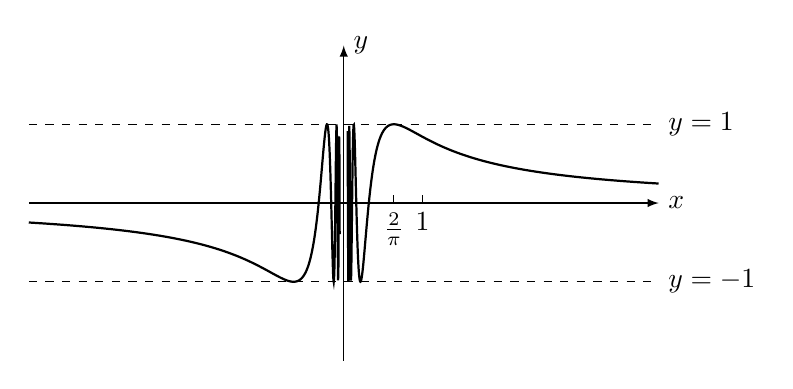
\begin{tikzpicture}[>=latex]
    \draw[->](-4,0)--(4,0)node[right]{$x$};
    \draw[->](0,-2)--(0,2)node[right]{$y$};
    \foreach \x in {1,-1}
    {
        \draw[dashed](-4,\x)--(4,\x)node[right]{$y=\x$};
    }
\draw[domain=-4:-.05, samples=1000, thick]plot(\x, {sin(180/pi/\x)});
\draw[domain=.05:4, samples=1000, thick]plot(\x, {sin(180/pi/\x)});
\foreach \x/\xtext in {1/1, .637/\frac{2}{\pi}}
{
    \draw(\x, 0)node[below]{$\xtext$}--(\x,.1);
}
\end{tikzpicture}    
    \caption{}
\end{figure}

上面是用数列的极限来说明函数的极限,其实我们也可以直接定义函数极限。

\begin{blk}{定义3}
  如果函数$f$在点$a$邻域上有定义(可能去掉点$a$本身),使得当$0<|x-a|<\delta$时,就有$|f(x)-\ell|<\varepsilon$, 那么就说$\ell$为当$x$趋近于$a$时,函数$f$在点$a$的极限值。
\end{blk}

我们对这个定义需要说明以下几点:
\begin{enumerate}
    \item 用定义3验证某数$\ell$是函数$f$在点$a$的极限的办法就是对于任给的$\varepsilon>0$, 要找到这样的正数$\delta$使得能够由不等式$|x-a|<\delta$推出不等式$|f(x)-\ell|<\varepsilon$,虽然$\varepsilon$是任意的正数,但是在找$\delta$的过程中,$\varepsilon$是固定不变的,$\delta$依赖于$\varepsilon$。
    \item 对于已给的$\varepsilon$, 只要证明有一个$\delta>0$存在就行.因为如果有一个$\delta$存在,把$\delta$再缩小一些,显然仍满足我们的要求。
    \item 不等式$|x-a|>0$只是说明$x\ne a$, 即把$x$等于$a$的情况去掉,这是因为我们关心的是函数$f$在点$a$附近的变化趋势,而和函数在$x=a$这点的值无关。
    \item 我们指出定义2和定义3是等价的.
\end{enumerate}

\begin{example}
用定义3证明$\Lim_{x\to 1}\frac{x^3-1}{x-1}=3$
\end{example}

\begin{proof}
    任给$\varepsilon>0$, 要找$\delta>0$, 使由$0<|x-1|<\delta$推出
    $\left|\frac{x^3-1}{x-1}-3\right|<\varepsilon$成立。

    当$x\ne 1$时,
\[\begin{split}
    \left|\frac{x^3-1}{x-1}-3\right|&=|(x^2+x+1)-3|\\
    &=|(x-1)(x+2)|=|x-1|\cdot |x-2|
\end{split}\]

要由$|x-1|\cdot |x+2|<\varepsilon$找$\delta$,显然,这里因子$|x+2|$引起了麻烦。为方便起见,先假定$0<|x-1|<1$,即取$\delta_1=1$,这样
\[0<|x-1|<1\quad\Rightarrow\quad |x+2|=|(x-1)+3|\le |x-1|+3<4\]因此,要使
\[\begin{cases}
    0<|x-1|<1\\
    |x-1|\cdot |x+2|<\varepsilon
\end{cases}\]
只须
\[\begin{cases}
    0<|x-1|<1\\
    4|x-1|<\varepsilon
\end{cases}\Rightarrow\quad \begin{cases}
    0<|x-1|<1\\
    |x-1|<\frac{\varepsilon}{4}
\end{cases}\]
由此可见,只须取$\delta=\min\left(1,\frac{\varepsilon}{4}\right)$,即取$\delta$为1与$\frac{\varepsilon}{4}$中的较小者。

$\therefore\quad $对于任意$\varepsilon>0$,取$\delta=\min\left(1,\frac{\varepsilon}{4}\right)$,则当$0<|x-1|<\delta$时,即有
\[\left|\frac{x^3-1}{x-1}-3\right|<\varepsilon\]
这也就证明了
\[\lim_{x\to 1}\frac{x^3-1}{x-1}=3\]
\end{proof}

\begin{example}
    证明$\Lim_{x\to a}\sqrt{x}=\sqrt{a}\quad (a>0)$
\end{example}

\begin{proof}
对于任意的$\varepsilon>0$, 我们必须找到一个$\delta>0$, 使得当$|x-a|<\delta$时,$|\sqrt{x}-\sqrt{a}|<\varepsilon$成立,因为
\[|\sqrt{x}-\sqrt{a}|=\frac{|x-a|}{\sqrt{x}+\sqrt{a}}<\frac{|x-a|}{\sqrt{a}}\]
所以要使$\frac{|x-a|}{\sqrt{a}}<\varepsilon$,只须$|x-a|<\sqrt{a}\varepsilon$

如果取$\delta=\sqrt{a}\varepsilon$,则$\frac{|x-a|}{\sqrt{a}}<\frac{\sqrt{a}\varepsilon}{\sqrt{a}}=\varepsilon$
因此,对于任意$\varepsilon>0$,取$\delta=\sqrt{a}\varepsilon$,则当$|x-a|<\delta$时,就有$|\sqrt{x}-\sqrt{a}|<\varepsilon$成立。这也就证明了
\[\lim_{x\to a}\sqrt{x}=\sqrt{a}\quad (a>0)\]
\end{proof}

有时虽然$f(x)$在某点的左边(或右边)没有定义,如图1.5中的$a,b$两点,我们也可以谈论$f$在点$a$或点$b$两点的极限,譬如对于所有小于$a$的数,$f$虽然没有定义,但是我们可以考察,当$x$从$a$的右侧趋近于$a$时,函数$f$的变化趋势,也就是考察$f$的单边极限是否存在。

\begin{figure}[htp]
    \centering
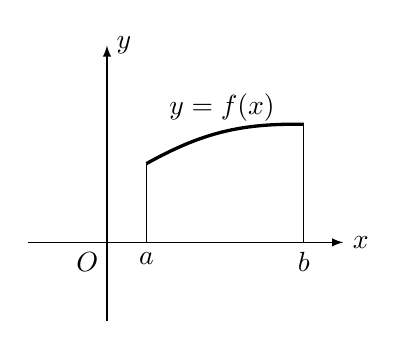
\begin{tikzpicture}[>=latex]
    \draw[->](-1,0)--(3,0)node[right]{$x$};
    \draw[->](0,-1)--(0,2.5)node[right]{$y$};
\draw[very thick](.5,1)to[bend right=-15]node[above]{$y=f(x)$} (2.5,1.5);
\draw(.5,1)--(.5,0)node[below]{$a$};
\draw(2.5,1.5)--(2.5,0)node[below]{$b$};
\node at (-.25,-.25){$O$};
\end{tikzpicture}
    \caption{}
\end{figure}

\begin{blk}{定义}
     设$f(x)$在区间$(a,b)$上有意义,如果任给$\varepsilon>0$, 总存在某个$\delta>0$使得当$x\in (a,a+\delta)$时,总有$|f(x)-\ell|<\varepsilon$,我们就说函数$f$在点$a$以$\ell$为\textbf{右极限},记作:
\[\lim_{x\to a^+}f(x)=\ell\]
\end{blk}

类似地,可以定义\textbf{左极限},只需把开区间$(a,a+\delta)$换成$(b-\delta,b)$就行了,并记作
\[\lim_{x\to b^-} f(x)=\ell\]

\begin{example}
    设函数$f(x)=\begin{cases}
        x-1,&x\le 1\\
x+1,&x>1
    \end{cases}\quad $    
    求$\Lim_{x\to 1^-}f(x)$和$\Lim_{x\to 1^+}f(x)$
\end{example}

\begin{figure}[htp]
    \centering
    \begin{minipage}[t]{0.48\textwidth}
    \centering
    \begin{tikzpicture}[>=stealth, scale=.6]
        \draw[->](-3,0)--(4,0)node[right]{$x$};
        \draw[->](0,-3)--(0,4.5)node[right]{$y$};
        \draw(0,1)node[left]{1}--(.1,1);
        \draw(0,2)node[left]{2}--(.1,2);
        \draw(1,0)node[below]{1}--(1,.1);
        \node at (-.25,-.25){$O$};
        \draw[domain=-2:1, samples=10, very thick]plot(\x,{\x-1});
        \draw[domain=1:3, samples=10, very thick]plot(\x,{\x+1});
    \node at (-2,-3)[left]{$y=x-1$};
    \node at (3,4)[right]{$y=x+1$};
    \draw[dashed](1,0)--(1,2)--(0,2);
    \draw (1,2)[fill=white] circle(2.5pt);
    
    \end{tikzpicture}
    \caption{}
    \end{minipage}
    \begin{minipage}[t]{0.48\textwidth}
    \centering
    \begin{tikzpicture}[>=stealth, scale=.8]
        \draw[->](-3,0)--(4,0)node[right]{$x$};
    \draw[->](0,-2.5)--(0,3)node[right]{$y$};
    \foreach \x in {-2,-1,1,2,3}
    {
        \draw(\x,0)node[below]{$\x$}--(\x,.1);
    }
\foreach \x in {-2,-1,1,2}
{
    \draw(0,\x)--(.1,\x)node[right]{$\x$};
}
\foreach \x in {-2,-1,...,2}
{
    \draw[very thick](\x,\x)--(\x+1,\x);
    \draw (\x+1,\x)[fill=white]circle(2pt);
}
    \node at (.25,-.25){$O$};
    \end{tikzpicture}
    \caption{}
    \end{minipage}
    \end{figure}


\begin{solution}
\[\begin{split}
    \lim_{x\to 1^-}f(x)&=\lim_{x\to 1^-}(x-1)=0\\
    \lim_{x\to 1^+}f(x)&=\lim_{x\to 1^+}(x+1)=2
\end{split}\]
图1.6显示了上面的结果。
\end{solution}

\begin{example}
    函数$y=[x]$代表不超过$x$的最大整数,即若$n\le x<n+1$,$n\in\mathbb{Z}$,则$y=[x]=n$。(图1.7)

求$\Lim_{x\to 2^+}\frac{[x]}{x},\quad \Lim_{x\to 2^-}\frac{[x]}{x}$
\end{example}





    









\begin{solution}
    显然,当$x=2$时,$\frac{[x]}{x}=\frac{[2]}{2}=\frac{2}{2}=1$, 又
\[\frac{[x]}{x}=\begin{cases}
    \frac{1}{x},& x\in(1,2)\\
    \frac{2}{x},& x\in(2,3)
\end{cases}\]
所以
\[\begin{split}
    \lim_{x\to 2^+}\frac{[x]}{x}&=\lim_{x\to 2^+}\frac{2}{x}=1\\
     \lim_{x\to 2^-}\frac{[x]}{x}&=\lim_{x\to 2^-}\frac{1}{x}=\frac{1}{2}
\end{split}\]    
\end{solution}


下面的命题说明函数的极限与函数的单边极限的关系:



\begin{example}

\end{example}

\begin{solution}
    
\end{solution}

    \begin{solution}
        
    \end{solution}
    